% Options for packages loaded elsewhere
\PassOptionsToPackage{unicode}{hyperref}
\PassOptionsToPackage{hyphens}{url}
%
\documentclass[
]{book}
\usepackage{lmodern}
\usepackage{amsmath}
\usepackage{ifxetex,ifluatex}
\ifnum 0\ifxetex 1\fi\ifluatex 1\fi=0 % if pdftex
  \usepackage[T1]{fontenc}
  \usepackage[utf8]{inputenc}
  \usepackage{textcomp} % provide euro and other symbols
  \usepackage{amssymb}
\else % if luatex or xetex
  \usepackage{unicode-math}
  \defaultfontfeatures{Scale=MatchLowercase}
  \defaultfontfeatures[\rmfamily]{Ligatures=TeX,Scale=1}
\fi
% Use upquote if available, for straight quotes in verbatim environments
\IfFileExists{upquote.sty}{\usepackage{upquote}}{}
\IfFileExists{microtype.sty}{% use microtype if available
  \usepackage[]{microtype}
  \UseMicrotypeSet[protrusion]{basicmath} % disable protrusion for tt fonts
}{}
\makeatletter
\@ifundefined{KOMAClassName}{% if non-KOMA class
  \IfFileExists{parskip.sty}{%
    \usepackage{parskip}
  }{% else
    \setlength{\parindent}{0pt}
    \setlength{\parskip}{6pt plus 2pt minus 1pt}}
}{% if KOMA class
  \KOMAoptions{parskip=half}}
\makeatother
\usepackage{xcolor}
\IfFileExists{xurl.sty}{\usepackage{xurl}}{} % add URL line breaks if available
\IfFileExists{bookmark.sty}{\usepackage{bookmark}}{\usepackage{hyperref}}
\hypersetup{
  pdftitle={EDS 221: Scientific Programming Essentials},
  pdfauthor={Allison Horst},
  hidelinks,
  pdfcreator={LaTeX via pandoc}}
\urlstyle{same} % disable monospaced font for URLs
\usepackage{color}
\usepackage{fancyvrb}
\newcommand{\VerbBar}{|}
\newcommand{\VERB}{\Verb[commandchars=\\\{\}]}
\DefineVerbatimEnvironment{Highlighting}{Verbatim}{commandchars=\\\{\}}
% Add ',fontsize=\small' for more characters per line
\usepackage{framed}
\definecolor{shadecolor}{RGB}{248,248,248}
\newenvironment{Shaded}{\begin{snugshade}}{\end{snugshade}}
\newcommand{\AlertTok}[1]{\textcolor[rgb]{0.94,0.16,0.16}{#1}}
\newcommand{\AnnotationTok}[1]{\textcolor[rgb]{0.56,0.35,0.01}{\textbf{\textit{#1}}}}
\newcommand{\AttributeTok}[1]{\textcolor[rgb]{0.77,0.63,0.00}{#1}}
\newcommand{\BaseNTok}[1]{\textcolor[rgb]{0.00,0.00,0.81}{#1}}
\newcommand{\BuiltInTok}[1]{#1}
\newcommand{\CharTok}[1]{\textcolor[rgb]{0.31,0.60,0.02}{#1}}
\newcommand{\CommentTok}[1]{\textcolor[rgb]{0.56,0.35,0.01}{\textit{#1}}}
\newcommand{\CommentVarTok}[1]{\textcolor[rgb]{0.56,0.35,0.01}{\textbf{\textit{#1}}}}
\newcommand{\ConstantTok}[1]{\textcolor[rgb]{0.00,0.00,0.00}{#1}}
\newcommand{\ControlFlowTok}[1]{\textcolor[rgb]{0.13,0.29,0.53}{\textbf{#1}}}
\newcommand{\DataTypeTok}[1]{\textcolor[rgb]{0.13,0.29,0.53}{#1}}
\newcommand{\DecValTok}[1]{\textcolor[rgb]{0.00,0.00,0.81}{#1}}
\newcommand{\DocumentationTok}[1]{\textcolor[rgb]{0.56,0.35,0.01}{\textbf{\textit{#1}}}}
\newcommand{\ErrorTok}[1]{\textcolor[rgb]{0.64,0.00,0.00}{\textbf{#1}}}
\newcommand{\ExtensionTok}[1]{#1}
\newcommand{\FloatTok}[1]{\textcolor[rgb]{0.00,0.00,0.81}{#1}}
\newcommand{\FunctionTok}[1]{\textcolor[rgb]{0.00,0.00,0.00}{#1}}
\newcommand{\ImportTok}[1]{#1}
\newcommand{\InformationTok}[1]{\textcolor[rgb]{0.56,0.35,0.01}{\textbf{\textit{#1}}}}
\newcommand{\KeywordTok}[1]{\textcolor[rgb]{0.13,0.29,0.53}{\textbf{#1}}}
\newcommand{\NormalTok}[1]{#1}
\newcommand{\OperatorTok}[1]{\textcolor[rgb]{0.81,0.36,0.00}{\textbf{#1}}}
\newcommand{\OtherTok}[1]{\textcolor[rgb]{0.56,0.35,0.01}{#1}}
\newcommand{\PreprocessorTok}[1]{\textcolor[rgb]{0.56,0.35,0.01}{\textit{#1}}}
\newcommand{\RegionMarkerTok}[1]{#1}
\newcommand{\SpecialCharTok}[1]{\textcolor[rgb]{0.00,0.00,0.00}{#1}}
\newcommand{\SpecialStringTok}[1]{\textcolor[rgb]{0.31,0.60,0.02}{#1}}
\newcommand{\StringTok}[1]{\textcolor[rgb]{0.31,0.60,0.02}{#1}}
\newcommand{\VariableTok}[1]{\textcolor[rgb]{0.00,0.00,0.00}{#1}}
\newcommand{\VerbatimStringTok}[1]{\textcolor[rgb]{0.31,0.60,0.02}{#1}}
\newcommand{\WarningTok}[1]{\textcolor[rgb]{0.56,0.35,0.01}{\textbf{\textit{#1}}}}
\usepackage{longtable,booktabs}
\usepackage{calc} % for calculating minipage widths
% Correct order of tables after \paragraph or \subparagraph
\usepackage{etoolbox}
\makeatletter
\patchcmd\longtable{\par}{\if@noskipsec\mbox{}\fi\par}{}{}
\makeatother
% Allow footnotes in longtable head/foot
\IfFileExists{footnotehyper.sty}{\usepackage{footnotehyper}}{\usepackage{footnote}}
\makesavenoteenv{longtable}
\usepackage{graphicx}
\makeatletter
\def\maxwidth{\ifdim\Gin@nat@width>\linewidth\linewidth\else\Gin@nat@width\fi}
\def\maxheight{\ifdim\Gin@nat@height>\textheight\textheight\else\Gin@nat@height\fi}
\makeatother
% Scale images if necessary, so that they will not overflow the page
% margins by default, and it is still possible to overwrite the defaults
% using explicit options in \includegraphics[width, height, ...]{}
\setkeys{Gin}{width=\maxwidth,height=\maxheight,keepaspectratio}
% Set default figure placement to htbp
\makeatletter
\def\fps@figure{htbp}
\makeatother
\setlength{\emergencystretch}{3em} % prevent overfull lines
\providecommand{\tightlist}{%
  \setlength{\itemsep}{0pt}\setlength{\parskip}{0pt}}
\setcounter{secnumdepth}{5}
\usepackage{booktabs}
\ifluatex
  \usepackage{selnolig}  % disable illegal ligatures
\fi
\usepackage[]{natbib}
\bibliographystyle{apalike}

\title{EDS 221: Scientific Programming Essentials}
\author{Allison Horst}
\date{2021-03-18}

\begin{document}
\maketitle

{
\setcounter{tocdepth}{1}
\tableofcontents
}
\hypertarget{scientific-programming-essentials-for-environmental-data-science}{%
\chapter{Scientific programming essentials for environmental data science}\label{scientific-programming-essentials-for-environmental-data-science}}


\includegraphics[width=0.5\linewidth]{images/bren_logo}

\hypertarget{material-disclaimer-and-use}{%
\subsection*{Material disclaimer and use}\label{material-disclaimer-and-use}}
\addcontentsline{toc}{subsection}{Material disclaimer and use}

This book was created by \href{www.allisonhorst.com}{Allison Horst} for EDS 221 (Scientific Programming Essentials) in the Master of Environmental Data Science program in the Bren School of Environmental Science and Management, UC Santa Barbara. It accompanies lecture, computational lab and discussion materials that may or may not be linked to throughout the book. This book is intended as a supplemental resource for some parts of the course. In other words, it is not intended as a standalone textbook.

All materials in this book are openly available for use and reuse by CC-BY.

\hypertarget{acknowledgement}{%
\subsection*{Acknowledgement}\label{acknowledgement}}
\addcontentsline{toc}{subsection}{Acknowledgement}

I create my courses by standing on shoulders of many giants in R, data science, and education communities. The wealth and quality of open educational resources (OERs) in data science has made teaching in the field fun, innovative, and inspiring. I've tried to thoroughly credit resources that I have pulled from and adapted for this book, and I welcome additions if I have missed any that should be included. Thanks, friends.

\hypertarget{course-introduction}{%
\section{Course introduction}\label{course-introduction}}

\begin{figure}

{\centering 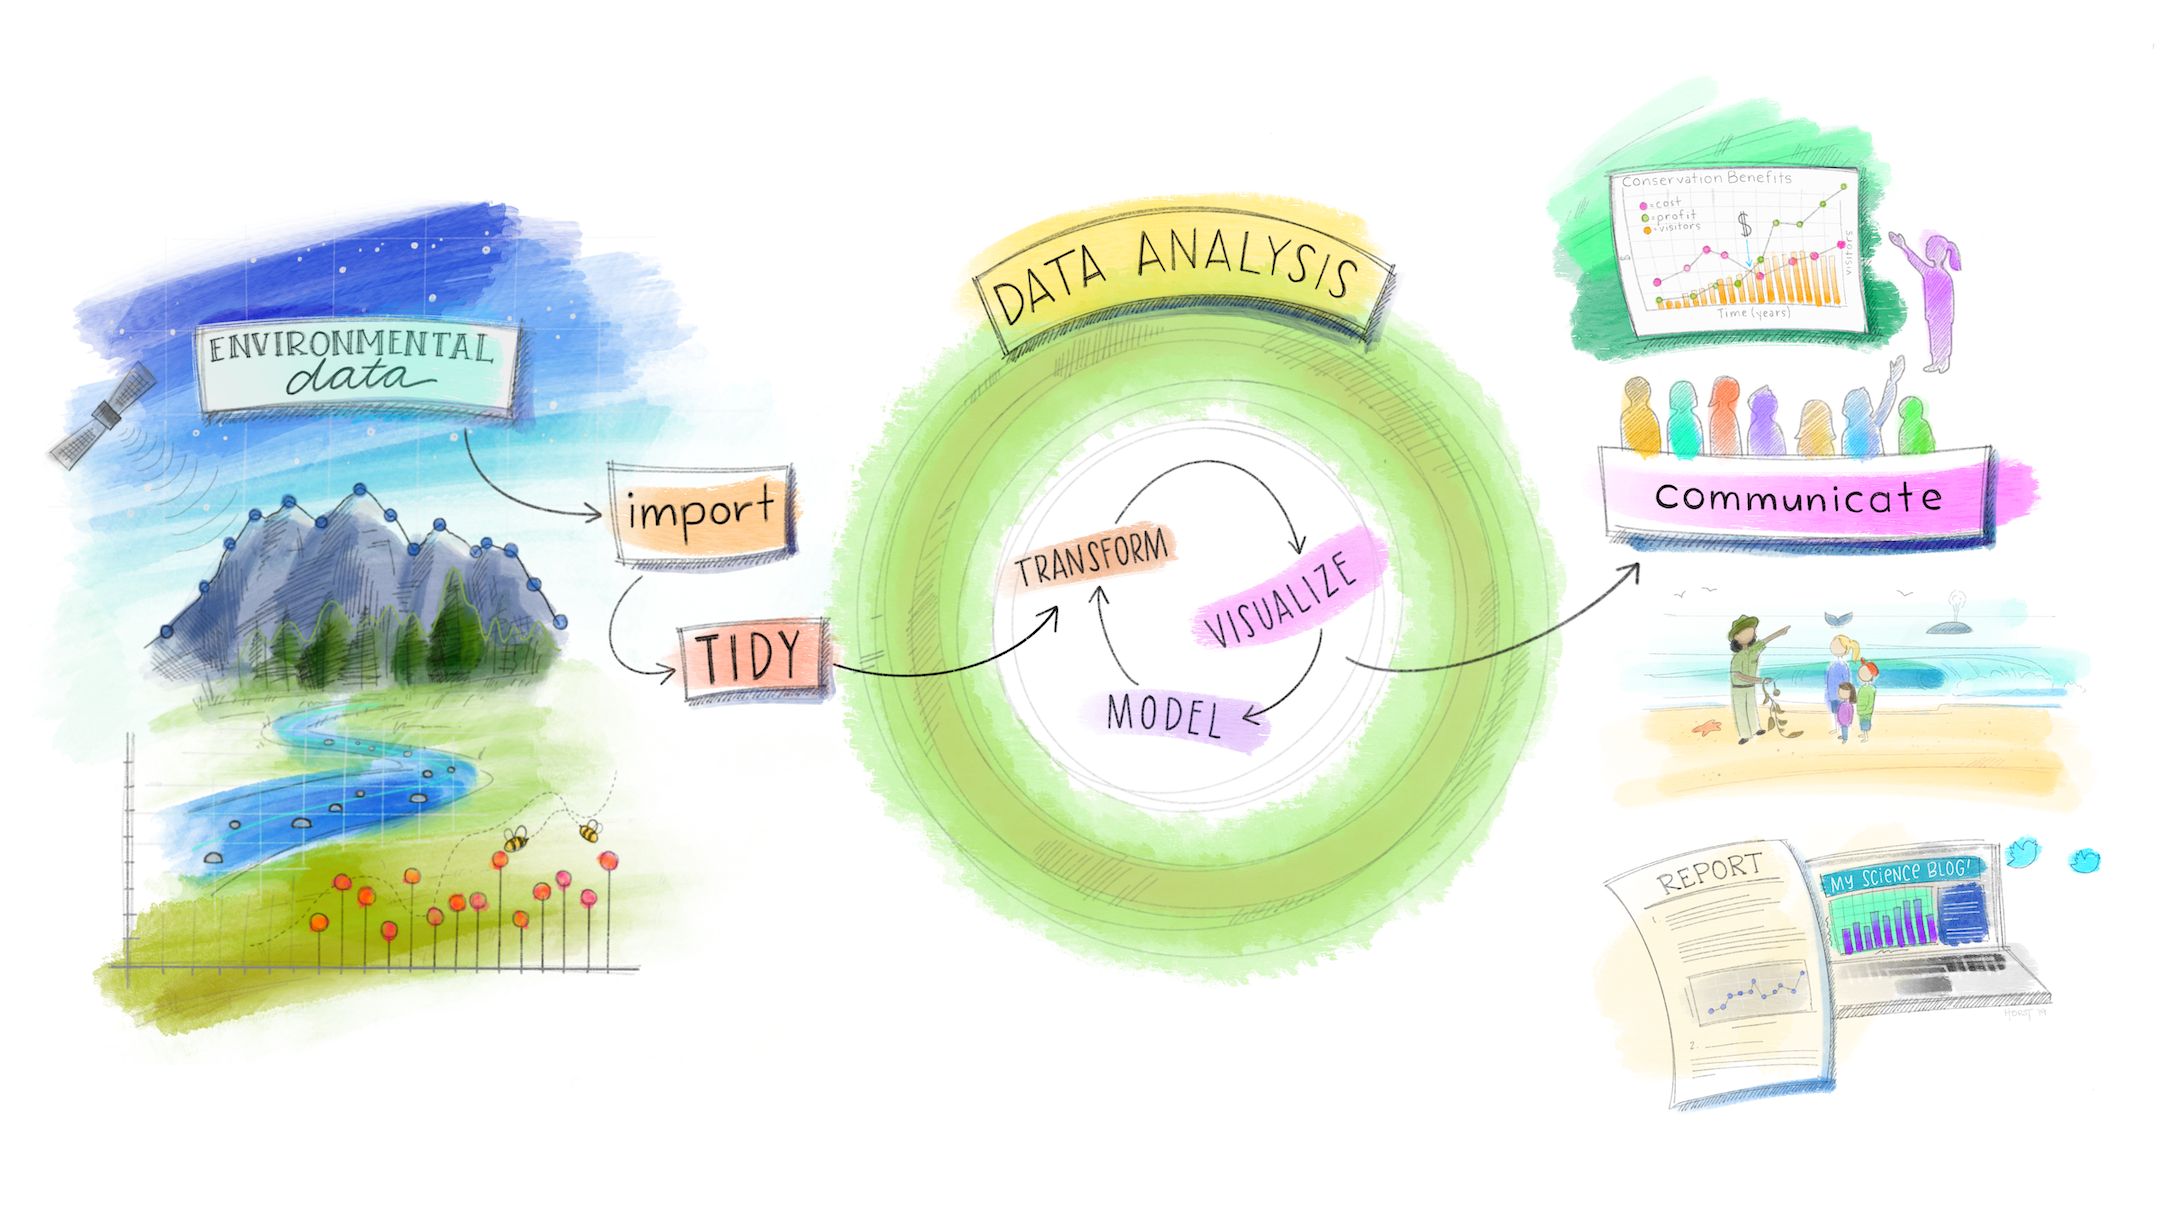
\includegraphics[width=1\linewidth]{images/eds_r4ds} 

}

\caption{Slide from Dr. Julia Lowndes' 2019 keynote talk at useR conference (illustration by Allison Horst).}\label{fig:unnamed-chunk-2}
\end{figure}

As nicely summarized in the title of a \href{https://www.nceas.ucsb.edu/news/next-generation-environmental-scientists-are-data-scientists}{2018 NCEAS post}: \emph{``The next generation of environmental scientists are data scientists''}.

Over the next year in MEDS you'll build skills to responsibly apply advanced methods in environmental modeling, spatial data analysis, and machine learning to investigate and solve environmental problems.

To get there, however, you'll need a strong foundation in programming basics like: understanding types and structures of data, basic data wrangling and visualization, algorithm development with functions, loops, and conditionals, and how to troubleshoot. While working in the weeds of programming, we'll also learn and reinforce transferable habits for reproducible workflows, robust file paths, version control, data organization, and more.

Upon these building blocks established in EDS 221, you'll be able to incrementally grow your advanced environmental data science toolkit to enter the workplace at the leading edge of quantitative methods in the field.

\hypertarget{setup}{%
\chapter{Setup}\label{setup}}

Intro to programming and the tools we're using.

\hypertarget{types}{%
\chapter{Data types and structures}\label{types}}

Data structures info\ldots{}

\hypertarget{methods}{%
\chapter{Methods}\label{methods}}

We describe our methods in this chapter.

\hypertarget{iteration}{%
\chapter{Iteration}\label{iteration}}

Iteration

\hypertarget{conditionals}{%
\chapter{Conditionals}\label{conditionals}}

\hypertarget{logicals}{%
\chapter{Logicals}\label{logicals}}

\hypertarget{functions}{%
\chapter{Functions}\label{functions}}

Writing functions to implement algorithms is a fundamental skill for every environmental data scientist. Functions can reduce repetition, increase efficiency and elegance, and facilitate reuse and sharing. Functions built by other developers will be ingrained into your code, but it's also critical that you can build, test, document, and share \textbf{your own} functions.

This chapter covers:

\begin{itemize}
\tightlist
\item
  Function structure
\item
  Writing basic functions
\item
  Nested functions
\item
  Functions with iteration and conditions
\item
  Useful function features
\item
  Testing
\item
  Documentation
\item
  Applied examples
\end{itemize}

\hypertarget{function-components}{%
\section{Function components}\label{function-components}}

At the most basic level, a function takes an input, does something to it (a calculation, transformation, etc.), and returns an output.

For example, we can write a function that doubles the input value. In \emph{function notation} seen in math, that would be:

\[f(x) = 2x\]
where \(x\) is the input, and \(f(x)\) is the output. The function \(f\) acts on input \(x\) by doubling the input value.

How can we create a function to do the same thing in R? An R function would look like this:

\begin{Shaded}
\begin{Highlighting}[]
\NormalTok{double\_it }\OtherTok{\textless{}{-}} \ControlFlowTok{function}\NormalTok{(x) \{}
  \DecValTok{2}\SpecialCharTok{*}\NormalTok{x}
\NormalTok{\}}
\end{Highlighting}
\end{Shaded}

What are these different pieces of that function?

\begin{itemize}
\tightlist
\item
  \texttt{double\_it}: this assigns the function a name which we'll need to use it later on.
\item
  \texttt{function(x)}: says we're making a function, and defines the function \textbf{formals} (arguments / parameters). This function expects a single input argument, \texttt{x} (you can check what the formals are using \texttt{formals(function\_name)}).
\item
  \texttt{\{\ 2*x\ \}}: the \textbf{body} of the function, where we tell it what to do with the inputs. Note the braces (i.e.~squiggly brackets).
\end{itemize}

Try out the function by inputting both a single value, and a vector of values. Note that vectorization is the default - meaning that the function is applied to each element in a vector.

\begin{Shaded}
\begin{Highlighting}[]
\FunctionTok{double\_it}\NormalTok{(}\AttributeTok{x =} \DecValTok{20}\NormalTok{)}
\end{Highlighting}
\end{Shaded}

\begin{verbatim}
## [1] 40
\end{verbatim}

\begin{Shaded}
\begin{Highlighting}[]
\NormalTok{vec }\OtherTok{\textless{}{-}} \FunctionTok{c}\NormalTok{(}\DecValTok{2}\NormalTok{, }\DecValTok{4}\NormalTok{, }\DecValTok{50}\NormalTok{) }\CommentTok{\# Create a vector with multiple values}

\FunctionTok{double\_it}\NormalTok{(vec) }\CommentTok{\# Function acts on each element in the vector}
\end{Highlighting}
\end{Shaded}

\begin{verbatim}
## [1]   4   8 100
\end{verbatim}

Those are the main pieces. But don't worry, it gets a lot more interesting. Let's start by writing a few of our own functions.

\hypertarget{writing-simple-functions}{%
\section{Writing simple functions}\label{writing-simple-functions}}

Let's practice writing a few simple functions using established relationships in environmental science.

\hypertarget{example-1-fish-standard-weight}{%
\subsection{Example 1: Fish standard weight}\label{example-1-fish-standard-weight}}

``Standard weight'' is how much we \emph{expect} a fish to weigh, give the species and fish length, and the nonlinear relationship is given by:

\[W=aL^b\]

where \(L\) is total fish length (centimeters), \(W\) is the expected fish weight (grams), and \(a\) and \(b\) are species-dependent parameter values.

Write a function to calculate fish weight based on \(a\), \(b\), and fish length, then estimate the weight of several fish based on the following parameter estimates for Hawaiian fish from Peyton et al.~(2015):

\begin{itemize}
\tightlist
\item
  \emph{Chanos chanos} (milkfish): \(a\) = 0.0905, \(b\) = 2.52
\item
  \emph{Sphyraena barracuda} (great barracuda): \(a\) = 0.0181, \(b\) = 3.27
\item
  \emph{Caranx ignobilis} (giant trevally): \(a\) = 0.0353, \(b\) = 3.05
\end{itemize}

Function:

\begin{Shaded}
\begin{Highlighting}[]
\NormalTok{predict\_weight }\OtherTok{\textless{}{-}} \ControlFlowTok{function}\NormalTok{(a, length, b) \{}
\NormalTok{  a}\SpecialCharTok{*}\NormalTok{(length}\SpecialCharTok{\^{}}\NormalTok{b)}
\NormalTok{\}}
\end{Highlighting}
\end{Shaded}

Using the function:

\begin{enumerate}
\def\labelenumi{\arabic{enumi}.}
\tightlist
\item
  Estimate the mass of a 160 cm long great barracuda.
\item
  Estimate the mass of a 118 cm long milkfish.
\end{enumerate}

\textbf{Thinking ahead:} how might we make this function simpler for a user? For example, maybe a user can input the \emph{species}, and the parameters \(a\) and \(b\) can be correctly updated for that species? We'll learn how to add this kind of functionality in upcoming sections.

\hypertarget{example-2}{%
\subsection{Example 2:}\label{example-2}}

\hypertarget{example-3}{%
\subsection{Example 3:}\label{example-3}}

\hypertarget{nested-functions}{%
\section{Nested functions}\label{nested-functions}}

\hypertarget{functions-with-iteration-and-conditionals}{%
\section{Functions with iteration and conditionals}\label{functions-with-iteration-and-conditionals}}

\hypertarget{useful-function-features}{%
\section{Useful function features}\label{useful-function-features}}

\hypertarget{testing-functions}{%
\section{Testing functions}\label{testing-functions}}

\hypertarget{iterating-functions}{%
\section{Iterating functions}\label{iterating-functions}}

\hypertarget{resources-on-building-testing-documenting-functions}{%
\section{Resources on building, testing, \& documenting functions}\label{resources-on-building-testing-documenting-functions}}

\begin{itemize}
\tightlist
\item
  \href{https://adv-r.hadley.nz/functions.html}{Ch. 6 - Functions} in \href{https://adv-r.hadley.nz/}{\emph{Advanced R}} by Hadley Wickham
\end{itemize}

\hypertarget{tidydata}{%
\chapter{Tidy data}\label{tidydata}}

\hypertarget{tidyverse}{%
\chapter{Data wrangling \& viz in the tidyverse}\label{tidyverse}}

\hypertarget{troubleshooting}{%
\chapter{Troubleshooting}\label{troubleshooting}}

  \bibliography{book.bib,packages.bib}

\end{document}
